% ----------
% A LaTeX template for course project reports
% 
% This template is modified from "Tech Report ala MIT AI Lab (1981)"
% 
% ----------
\documentclass[12pt, letterpaper, twoside]{article}
\usepackage{geometry}
\usepackage[utf8]{inputenc}
\usepackage[english]{babel}
\usepackage[runin]{abstract}
\usepackage{titling}
\usepackage{booktabs}
% Source - https://stackoverflow.com/a/2739710
% Posted by Mica, modified by community. See post 'Timeline' for change history
% Retrieved 2026-02-08, License - CC BY-SA 3.0
\usepackage{pdfpages}
\usepackage{fancyhdr}
\usepackage{helvet}
\usepackage{csquotes}
\usepackage{graphicx}
\usepackage{blindtext}
\usepackage{parskip}
\usepackage{etoolbox}


\input{preamble.tex}

% ----------
% Variables
% ----------

\title{\textbf{{\LARGE Assignment \#02 — Smart Drone Hangar}} \\ {\ Course: Embedded Systems and Internet of Things}} % Full title of your tech report
\runningtitle{Ass. \#02 — SDH} % Short title
\author{Nicholas Magi \\ \texttt{0001113915} \and Rebecca Scarcelli \\ \texttt{0001118585} \and Elettra Ventura \\ \texttt{0001117272}} % Full list of authors
\runningauthor{N. Magi, R. Scarcelli, E. Ventura} % Short list of authors
\affiliation{University of Bologna, Cesena Campus} % Affiliation e.g. University or Company
\department{Department of Computer Science and Engineering} % Department or Office
\theyear{2026} % year of the tech report
\mydate{February 5, 2026} %the date


% ----------
% actual document
% ----------
\begin{document}
\maketitle

\begin{abstract}
    The assignment requires the development of a Smart Drone Hangar system using Arduino along with high abstract concepts such as FSM (Finite State Machines) and Task-based architecture. This document is meant to provide a detailed description about our work, how we implemented the Smart Drone Hangar (SDH) and the Drone Remote Unit (DRU) and how we made them communicate.
\end{abstract}

\vspace{2.5cm}

% Uncomment the following to add thanks.
% {\footnotesize
%     \noindent
%     Special thanks to \textbf{Person 1} and \textbf{Affiliation A} for financial support for this project.
% }

\thispagestyle{firstpage}

\pagebreak

% ----------
% End of first page
% ----------

\newgeometry{} % Redefine geometries (normal margins)

\tableofcontents

\pagebreak

\section{Introduction}
\label{sec:intro}

\subsection{Requirements — v1.1.1-20251112}
 
We want to realise an embedded system called \textit{Smart Drone Hangar}. The prototype  is meant to implement a simple smart hangar for a drone. 

\begin{figure}[h]
    \centering
    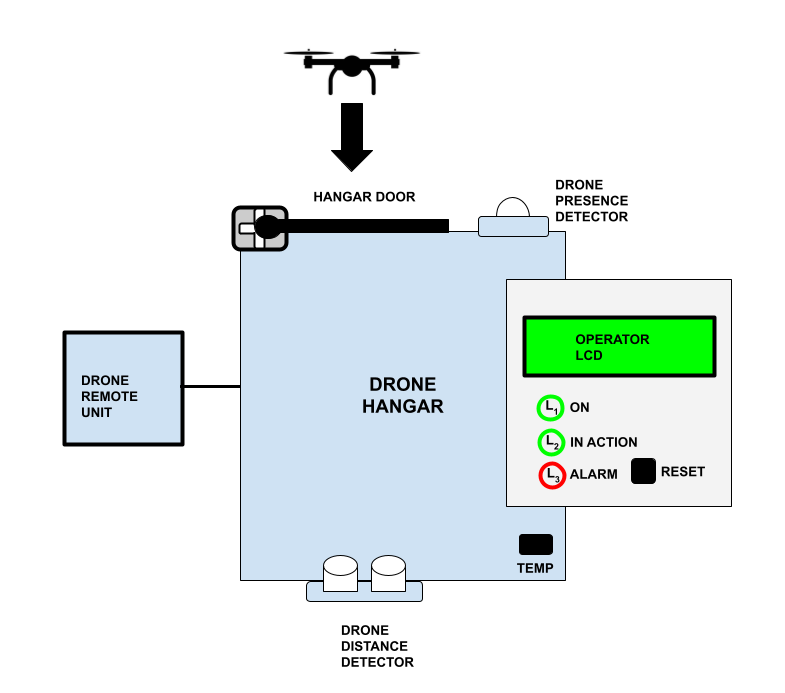
\includegraphics[width=0.5\linewidth]{assets/imgs/assignment-02-sketch.png}
    \caption{Suggested layout}
    \label{fig:placeholder}
\end{figure}

\subsubsection{Description - Components}

The system is composed by two subsystems:

\begin{itemize}
    \item \textbf{DRONE HANGAR} subsystem, based on Arduino 
    \begin{itemize}
        \item \textbf{DRONE PRESENCE DETECTOR (DPD)} is a PIR, to detect the presence of a drone near (on top) of the hangar.
        \item \textbf{DRONE DISTANCE DETECTOR (DDD)} is a sonar, to measure the distance of the drone when it is inside the hangar.
        \item \textbf{HANGAR DOOR (HD)} is a servo-motor, controlling the hangar door.
        \item \textbf{OPERATOR LCD} is a I2C LCD, used to interact with an operator.
        \item \textbf{L1} and \textbf{L2} are green leds, \textbf{L3} is a red led.
        \item \textbf{RESET} is a tactile button.
        \item \textbf{TEMP} is an analog temperature sensor.
    \end{itemize}
    \item \textbf{DRONE REMOTE UNIT (DRU)} (PC-based):
    \begin{itemize}
        \item A GUI-based subsystem that simulates a bridge to the drone to send/receive commands.
        \item Communicates via \textbf{serial line} with the DRONE HANGAR subsystem.
    \end{itemize}
\end{itemize}  

\subsubsection{Description - Behaviour}

At startup, the \textbf{HD} door is closed, and the drone is assumed to be inside at rest. \textbf{L1} is ON, \textbf{L2} and \textbf{L3} are OFF, and the LCD displays \texttt{DRONE INSIDE}.

\paragraph{Take-off phase}
The drone sends an opening command via the \textbf{DRU}. Upon reception:
\begin{enumerate}
    \item \textbf{HD} opens and the LCD displays \texttt{TAKE OFF}.
    \item The system monitors \textbf{DDD}.
    \item When measured distance $> D1$ for more than $T1$ seconds, the drone is assumed to have exited.
    \item \textbf{HD} closes and the LCD displays \texttt{DRONE OUT}.
\end{enumerate}

\paragraph{Landing phase}
The drone sends an opening command via \textbf{DRU}. 
\begin{enumerate}
    \item If \textbf{DPD} detects the drone, \textbf{HD} opens and the LCD displays \texttt{LANDING}.
    \item The system monitors \textbf{DDD}.
    \item When distance $< D2$ for more than $T2$ seconds, the drone is assumed to have landed.
    \item \textbf{HD} closes and the LCD displays \texttt{DRONE INSIDE}.
\end{enumerate}

During the take-off and landing phases, \textbf{L2} blinks, with period 0.5 second -- otherwise it is off.

Temperature monitoring is active whenever the drone is inside or in transition:
\begin{itemize}
    \item \textbf{Pre-alarm}: If $Temp \geq Temp1$ for $> T3$ seconds, new operations are suspended. Ongoing operations are allowed to finish. The system recovers if temperature drops below $Temp1$.
    \item \textbf{Alarm}: If $Temp \geq Temp2$ for $> T4$ seconds (where $Temp2 > Temp1$):
    \begin{enumerate}
        \item \textbf{HD} is closed immediately.
        \item \textbf{L3} turns ON and LCD displays \texttt{ALARM}.
        \item If the drone is outside, an \texttt{ALARM} message is sent via \textbf{DRU}.
        \item All operations are suspended until the \textbf{RESET} button is pressed.
    \end{enumerate}
\end{itemize}

The value of the \texttt{D1}, \texttt{D2}, \texttt{T1}, \texttt{T2}, \texttt{T3}, \texttt{T4}, \texttt{Temp1}, \texttt{Temp2} parameters is not fixed/specified (to be chosen, useful for prototyping/testing the system).

Develop the software using a \textbf{task-based architecture} and \textbf{synchronous Finite State Machines (FSM)} for the Arduino part. The PC part (DRU) must feature a GUI to:
\begin{itemize}
    \item Send simulation commands (Take-off/Landing).
    \item Visualize drone state (Rest, Taking off, Operating, Landing).
    \item Visualize hangar state (Normal, Alarm).
    \item Display real-time distance during landing.
\end{itemize}

For any aspect not specified, you are free to choose the approach you consider more useful or valuable.

\subsubsection{Description - the deliverable}

The deliverable consists in a zipped folder \texttt{assignment-02.zip} including three directories:
\begin{itemize}
    \item \texttt{drone-hangar}, including the source code of the Arduino-based subsystem
    \item \texttt{drone-remote-unit}, including the source code of the PC-based part
    \item \texttt{doc}, including: a brief \textbf{report} describing the solution, in particular the diagram of the FSMs and the  representation of the schema/breadboard – using tools such as TinkerCad or Fritzing , and a \textbf{short video} (or the link to a video on the UNIBO OneDrive cloud) demonstrating the system. 
\end{itemize}


\section{Smart Drone Hangar}

\subsection{How to run the program}

\subsection{Task-based architecture}
When looking at the assignment description, our first focus was to try to define the tasks hidden in it — in order to decompose and modularize the system. Much attention was put on the Smart Drone Hangar subsystem, since it is designed to be implemented using a \textbf{task-based architecture}.

From a theoretical point of view, we can recall that a task is defined as a \textit{single well-defined unit of work/job to be done}, and that the behaviour of each task can be represented by a \textbf{finite-state machine}. \\
A \textbf{state machine} is no other than a general model of a system with discrete dynamics that at \textit{each reaction maps valuation of the inputs to valuations of the outputs, where the map may depend on its current state}. \\
A \textbf{finite-state machine} is a state machine whose set of possible states is finite (\textit{i.e. has a finite number of elements}).

\subsubsection{UML State Diagram of the Finite State Machines}
% Source - https://stackoverflow.com/a/2739710
% Posted by Mica, modified by community. See post 'Timeline' for change history
% Retrieved 2026-02-08, License - CC BY-SA 3.0


\includepdf[pages=-,scale=.9]{assets/FSM-SDH.pdf}

Starting from the general problem, we considered two subsystems: the Smart Hangar and the temperature monitoring system embedded in it. They both share two global variables: \texttt{isAlarm} and \texttt{canFly}. They determine whether the temperature monitoring system is in \texttt{ALARM} state and whether the drone can begin new take off or landing operations, respectevely.

\subsubsection{Smart Hangar states}
We designed all the states of the Smart Hangar according to the position of the drone relative to it.
\begin{enumerate}
    \item \texttt{DRONE INSIDE} \\
    The starting point of the Smart Hangar system.
    \item \texttt{TAKE OFF} \\
    When the DRU (Drone Remote Unit) communicates the hangar it wants to take off, the hangar opens the door and waits for the drone to exit.
    \item \texttt{DRONE OUT} \\
    When the drone is operating outside the hangar and is distant enough from it, the hangar closes the door.
    \item \texttt{LANDING} \\
    Once the flying drone wants to land, it sends a message via DRU to the hangar. At that point, the hangar opens the door and waits for the drone to land.
\end{enumerate}

At any point in time during the execution of the system, the hangar can enter the \texttt{ALARM} state: in this state new take offs and landings are suspended, while the drone is allowed to finish its current take off/landing.

\subsubsection{Temperature monitoring system states}

\section{Drone Remote Unit}

\subsection{How to run the program}

\label{sec:conc}

% Uncomment following to add an acknowledgement section
% \section*{Acknowledgements}

% Thanks again to \textbf{Person 1} and \textbf{Affiliation A} for their financial support.

% ----------
% Bibliography
% ----------

% Uncomment the following and add your references into biblio.bib file
% \bibliography{./biblio.bib}
% \bibliographystyle{abbrv}

\end{document}

% ----------
